\documentclass[UTF8,a4paper,10pt]{ctexart}
\usepackage[left=3.17cm, right=3.17cm, top=2.74cm, bottom=2.74cm]{geometry}
\usepackage{amsmath}
\usepackage{graphicx,subfig}
\usepackage{float}
\usepackage{cite}
\usepackage{caption}
\usepackage{enumerate}
\usepackage{booktabs} %表格
\usepackage{multirow}
\newcommand{\tabincell}[2]{\begin{tabular}{@{}#1@{}}#2\end{tabular}}  %表格强制换行
%-------------------------字体设置--------------
\usepackage{times} 
\setmainfont{TimesNewRomanPSMT}%英文一律使用times new roman
%楷体\kaishu  黑体\heiti 仿宋\fangsong 隶书\lishu  幼圆\youyuan
% \setCJKmainfont[BoldFont=Kaiti SC Bold]{Kaiti SC}   %大概是唯一一个有粗体的楷体_(:з」∠)_
\setCJKfamilyfont{kt}[BoldFont=Kaiti SC Bold]{Kaiti SC}
\newcommand{\kt}{\CJKfamily{kt}}  
\newcommand{\song}{\CJKfamily{song}}    % 宋体
\newcommand{\fs}{\CJKfamily{fs}}             % 仿宋体
\setCJKfamilyfont{hwkt}{STKaiti} %引用华文楷体
\newcommand{\hwkt}{\CJKfamily{hwkt}} 
\setCJKfamilyfont{hwxk}{STXingkai} %引用华文行楷
\newcommand{\hwxk}{\CJKfamily{hwxk}}
\newcommand{\yihao}{\fontsize{26pt}{36pt}\selectfont}           % 一号, 1.4 倍行距
\newcommand{\erhao}{\fontsize{22pt}{28pt}\selectfont}          % 二号, 1.25倍行距
\newcommand{\xiaoer}{\fontsize{18pt}{18pt}\selectfont}          % 小二, 单倍行距
\newcommand{\sanhao}{\fontsize{16pt}{24pt}\selectfont}  %三号字
\newcommand{\xiaosan}{\fontsize{15pt}{22pt}\selectfont}        % 小三, 1.5倍行距
\newcommand{\sihao}{\fontsize{14pt}{21pt}\selectfont}            % 四号, 1.5 倍行距
\newcommand{\banxiaosi}{\fontsize{13pt}{19.5pt}\selectfont}    % 半小四, 1.5倍行距
\newcommand{\xiaosi}{\fontsize{12pt}{18pt}\selectfont}            % 小四, 1.5倍行距
\newcommand{\dawuhao}{\fontsize{11pt}{11pt}\selectfont}       % 大五号, 单倍行距
\newcommand{\wuhao}{\fontsize{10.5pt}{15.75pt}\selectfont}    % 五号, 单倍行距
%-------------------------章节名----------------
\usepackage{ctexcap} 
\CTEXsetup[name={,、},number={ \chinese{section}}]{section}
\CTEXsetup[name={(,)},number={\chinese{subsection}}]{subsection}
\CTEXsetup[name={,.},number={\arabic{subsubsection}}]{subsubsection}
%-------------------------页眉页脚--------------
\usepackage{fancyhdr}
\pagestyle{fancy}
\lhead{\kaishu \leftmark}
% \chead{}
\rhead{\kaishu 系统综合课程设计实验报告}%加粗\bfseries 
\lfoot{}
\cfoot{\thepage}
\rfoot{}
\renewcommand{\headrulewidth}{0.1pt}  
\renewcommand{\footrulewidth}{0pt}%去掉横线
\newcommand{\HRule}{\rule{\linewidth}{0.5mm}}%标题横线
\newcommand{\HRulegrossa}{\rule{\linewidth}{1.2mm}}
%-----------------------伪代码------------------
\usepackage{algorithm}  
\usepackage{algorithmicx}  
\usepackage{algpseudocode}  
\floatname{algorithm}{Algorithm}  
\renewcommand{\algorithmicrequire}{\textbf{Input:}}  
\renewcommand{\algorithmicensure}{\textbf{Output:}} 
\usepackage{lipsum}  
\makeatletter
\newenvironment{breakablealgorithm}
  {% \begin{breakablealgorithm}
   \begin{center}
     \refstepcounter{algorithm}% New algorithm
     \hrule height.8pt depth0pt \kern2pt% \@fs@pre for \@fs@ruled
     \renewcommand{\caption}[2][\relax]{% Make a new \caption
       {\raggedright\textbf{\ALG@name~\thealgorithm} ##2\par}%
       \ifx\relax##1\relax % #1 is \relax
         \addcontentsline{loa}{algorithm}{\protect\numberline{\thealgorithm}##2}%
       \else % #1 is not \relax
         \addcontentsline{loa}{algorithm}{\protect\numberline{\thealgorithm}##1}%
       \fi
       \kern2pt\hrule\kern2pt
     }
  }{% \end{breakablealgorithm}
     \kern2pt\hrule\relax% \@fs@post for \@fs@ruled
   \end{center}
  }
\makeatother
%------------------------代码-------------------
\usepackage{xcolor} 
\usepackage{listings} 
\lstset{ 
basicstyle=\small,
escapeinside=``,
keywordstyle=\color{ blue!70} \bfseries,
commentstyle=\color{red!50!green!50!blue!50},% 
stringstyle=\ttfamily,% 
extendedchars=false,% 
linewidth=\textwidth,% 
numbers=left,% 
numberstyle=\tiny \color{blue!50},% 
frame=trbl% 
rulesepcolor= \color{ red!20!green!20!blue!20} 
}
%------------超链接----------
\usepackage[colorlinks,linkcolor=black,anchorcolor=blue]{hyperref}
%------------------------TODO-------------------
\usepackage{enumitem,amssymb}
\newlist{todolist}{itemize}{2}
\setlist[todolist]{label=$\square$}
% for check symbol 
\usepackage{pifont}
\newcommand{\cmark}{\ding{51}}%
\newcommand{\xmark}{\ding{55}}%
\newcommand{\done}{\rlap{$\square$}{\raisebox{2pt}{\large\hspace{1pt}\cmark}}\hspace{-2.5pt}}
\newcommand{\wontfix}{\rlap{$\square$}{\large\hspace{1pt}\xmark}}
%------------------------水印-------------------
\usepackage{tikz}
\usepackage{xcolor}
\usepackage{eso-pic}

\newcommand{\watermark}[3]{\AddToShipoutPictureBG{
\parbox[b][\paperheight]{\paperwidth}{
\vfill%
\centering%
\tikz[remember picture, overlay]%
  \node [rotate = #1, scale = #2] at (current page.center)%
    {\textcolor{gray!80!cyan!30!magenta!30}{#3}};
\vfill}}}
%----------------------------------------------
\begin{document}
\begin{titlepage}
    \begin{center}
    
\includegraphics[width=0.8\textwidth]{fig/NKU.png}\\[1cm]    
    \textsc{\Huge \kaishu{\textbf{南\ \ \ \ \ \ 开\ \ \ \ \ \ 大\ \ \ \ \ \ 学}} }\\[0.9cm]
    \textsc{\huge \kaishu{\textbf{计\ \ 算\ \ 机\ \ 学\ \ 院}}}\\[0.5cm]
    \textsc{\Large \textbf{系统综合课程设计实验报告}}\\[0.8cm]
    \HRule \\[0.9cm]
    { \LARGE \bfseries PA3实验报告}\\[0.4cm]
    \HRule \\[2.0cm]
    \centering
    \textsc{\LARGE \kaishu{\ \ \ \ 周辰霏1712991}}\\[0.5cm]
    \textsc{\LARGE \kaishu{年级\ :\ 2017级}}\\[0.5cm]
    \textsc{\LARGE \kaishu{专业\ :\ 计算机科学与技术}}\\[0.5cm]
    \vfill
    {\Large \today}
    \end{center}
\end{titlepage}
%----------------------------------------没想好摘要写什么不写了-----------------------------------------------------------
% \newpage
% \thispagestyle{empty}
% \renewcommand{\abstractname}{\kaishu \sihao \textbf{摘要}}
%     \begin{abstract}
%         \kt{实现基于Phong模型的光线跟踪渲染器,实现全部基础功能以及任意obj文件的渲染和纹理的附加功能。 

%         在此附上\href{https://github.com/TiffanyChou21/COSC-0035-CG/tree/master/Phong}{GitHub仓库}以及\href{https://cdn.jsdelivr.net/gh/TiffanyChou21/CDN/video/Phong.mp4}{演示Demo}  }   
%         \noindent  %顶格
%         \kt{\textbf{\\\ 关键字:}\textbf{Phong模型;光线跟踪;蒙特卡罗;C++} \\\ \\\ } 
%     \end{abstract}
%---------------------------------------------------------------------------------------------------
\tableofcontents
%---------------------------------------------------------------------------------------------------
\newpage
\watermark{60}{10}{PA3}
\setcounter{page}{1}
\section{概述}
%——————————————————————————————————————
\subsection{实验目的}
\kt{
    \begin{itemize}
        \item 梳理操作系统概念
        \item 学习系统调用,并实现中断机制
        \item 了解文件系统的基本内容,实现简易文件系统
        \item 实现支持文件操作的操作系统,要求能成功运行仙剑奇侠传
    \end{itemize}

    PA3完成的内容和标题一样——批处理系统,基本上实现了除了内存管理和进程管理(PA4)以外的其他基本功能,尤以中断和系统调用为最,贯穿整个PA3始终。整体而言完成了中断异常处理,系统调用相关之后底层基础已经打好了,再利用这些实现输出和文件系统(极简化)后就可以加载pal开始剧情的享受了。最后还有一部分基础设施的完善内容——DiffTest的自由调试开关控制。
}
%——————————————————————————————————————
\subsection{实验内容}
\kt{
    PA3实验涉及现代指令系统的实现、抽象机器AM 的原理与应用、输入输出设备三部分
    \begin{enumerate}
        \item 熟悉操作系统的基本概念、系统调用,实现子线操作\_yield(),这其中包括异常的发现和处理以及CTE上下文的保存和恢复
        \item 实现用户程序的加载和系统调用, 支撑TRM程序的运行
        \item 运行仙剑奇侠传并展示批处理系统, 包括文件系统的实现
        \item 对DiffTest实现自由开关以自行选择DiffTest进行调试的代码部分
    \end{enumerate}
}
%---------------------------------------------------------------------------------------------------
\section{阶段一}
%——————————————————————————————————————
\subsection{了解Nanos-lite}
\kt{
  可以把Nanos-lite理解成一个运行在AM上的特殊的应用程序,它协助我们管理和运行其他应用程序。阅读main.c了解当前Nanos-lite都做了些什么,输出编译信息、初始化磁盘(一段内存)、设备初始化(IOE)、初始化文件以及进程(PA4的内容)、调用panic结束Nanos-lite。

  而当我们在common.h里面取消对HAS\_CTE的注释以后,Nanos-lite就会在panic之前调用\_yield()以触发自陷操作,在这之前还会先对CTE上下文进行初始化:初始化IDT并对其内容进行设置使其有意义,之后设置一个处理回调函数,我们可以用这个来处理事件。
}
%——————————————————————————————————————
\subsection{中断触发}
\kt{
  中断实际上由触发中断、保存上下文、切换内核模式、根据中断号对其进行处理、恢复上下文组成。实现自陷操作先从\_yield()看起,指导书提到了IDT的设置中需要使用lidt指令,而在cte.c中定义的yield实际上是借助x86中的int指令引发一个中断来让中断例程对中断进行处理,那么显然我们需要实现int指令。两个命令都在system.c中,还是和PA2一样的实现即可。由于加入了新的内容,所以需要在reg.h中对IDTR进行声明,同时为了DiffTest的对照还要加入一个CS寄存器。为了配合DiffTest的运行,eflags和CS都需要在restart函数中进行相应初始化。int指令是对触发int之前的eip进行处理,而非当前eip;而lidt指令是对id\_dest的地址进行操作。
  \begin{lstlisting}[title=int-lidt实现,frame=trbl,language={C++}]
    //nemu/src/isa/x86/exec/exec.c
    /* 0x0f 0x01*/
    make_group(gp7,
        EMPTY, EMPTY, EMPTY, EX(lidt),
        EMPTY, EMPTY, EMPTY, EMPTY)
    /* 0xcc */	EMPTY, IDEXW(I,int,1), EMPTY, EX(iret),
    //nemu/src/isa/x86/include/isa/reg.h
    struct 
    {
      uint16_t limit;
      uint32_t base;
    }IDTR;
    rtlreg_t CS; 
    //nemu/src/isa/x86/exec/system.c
    make_EHelper(int) {
      raise_intr(id_dest->val,decoding.seq_eip); //之前的eip
      print_asm("int %s", id_dest->str);

      #ifdef DIFF_TEST
        diff_test_skip_nemu();
      #endif
    }
    make_EHelper(lidt) {
      rtl_li(&t0,id_dest->addr);//不是id_dest->val!!!
      rtl_li(&cpu.IDTR.limit,vaddr_read(t0,2));
      rtl_li(&cpu.IDTR.base,vaddr_read(t0+2,4));
      print_asm_template1(lidt);
    }
    //nemu/src/isa/x86/init.c
    static void restart() {
      /* Set the initial program counter. */
      cpu.pc = PC_START;
      cpu.CS=8;
      cpu.eflags.flags=0x2;
    }
  \end{lstlisting}

  前面准备工作都做好之后,就可以实现raise\_intr()函数了,raise\_intr()函数实际上是根据中断号对中断进行标记追踪处理,在跳转到新的地址的同时保存当前cpu的状态。
  \begin{lstlisting}[title=raise\_intr(),frame=trbl,language={C++}]
    //nemu/src/isa/x86/init/intr.c
void raise_intr(uint8_t NO, vaddr_t ret_addr) {
  /* TODO: Trigger an interrupt/exception with ``NO''.
   * That is, use ``NO'' to index the IDT.
   */
  //当前状态压栈保存
  rtl_push(&cpu.eflags.flags);
  cpu.eflags.IF = 0;
  rtl_push(&cpu.cs);
  rtl_push(&ret_addr);
  //读出IDTR首地址,找到们描述符
  rtl_li(&t0,vaddr_read(cpu.idtr.i_base+8*NO,4));
  rtl_li(&t1,vaddr_read(cpu.idtr.i_base+8*NO+4,4));
  //合成目标地址并跳转
  rtl_j(t0|t1);
}
  \end{lstlisting}
}
%——————————————————————————————————————
\subsection{保存上下文}
\kt{
  之后根据cte.c,异常入口被设定为vectrap(trap.S实现),它调用了irq\_handle()对事件进行处理。当然暂时我们并不需要关心这个,因为此时$run$以后我们发现有未实现命令的出现,这个命令实际上是pusha,而它是在保存上下文中起作用保存压栈寄存器的值。
  \begin{lstlisting}[title=pusha指令,frame=trbl,language={C++}]
//nemu/src/isa/x86/exec/exec.c
/* 0x60 */	EX(pusha), EX(popa), EMPTY, EMPTY,
make_EHelper(pusha) {
  t0 = cpu.esp;
  rtl_push(&cpu.eax);
  rtl_push(&cpu.ecx);
  rtl_push(&cpu.edx);
  rtl_push(&cpu.ebx);
  rtl_push(&t0);
  rtl_push(&cpu.ebp);
  rtl_push(&cpu.esi);
  rtl_push(&cpu.edi);
  print_asm("pusha");
}
  \end{lstlisting}

  之后需要重构\_Context中的顺序使其和前面trap.S中构造的一致,实际上只要和pusha压栈的顺序一致,保证压栈正确即可。上下文的全部组成就是八个通用寄存器以及eip、cs和eflags。
  \begin{lstlisting}[title=Context,frame=trbl,language={C++}]
//nexus-am/am/include/arch/x86-nemu.h
struct _Context {
  struct _AddressSpace *as;
  uintptr_t edi,esi,ebp,esp,ebx,edx,ecx,eax;
  int irq;
  uintptr_t eip,cs,eflags;
};
  \end{lstlisting}
}
%——————————————————————————————————————
\subsection{事件打包分发}
\kt{ 
  在上下文保存好之后,OS就会进入内核态并根据中断号来进行相应的中断处理,而这就是我们下来要做的打包事件并使用回调函数通过OS进行处理。在PA里面我们只需要在cte.c里面对事件识别并打包,然后在irq.c里面对对应编号事件进行处理即可。
  \begin{lstlisting}[title=irq,frame=trbl,language={C++}]
//nexus-am/am/src/x86/nemu/cte.c
_Context* __am_irq_handle(_Context *c) {
  _Context *next = c;
  if (user_handler) {
    _Event ev = {0};
    switch (c->irq) {
      case 0x81:ev.event=_EVENT_YIELD;break;//int 81
      default: ev.event = _EVENT_ERROR; break;
    }
    next = user_handler(ev, c);
    if (next == NULL) {
      next = c;
    }
  }
  return next;
}
//nanos-lite/src/irq.c
static _Context* do_event(_Event e, _Context* c) {
  switch (e.event) {
    case _EVENT_YIELD:printf("system yeild\n");break;//识别yield事件并输出一句话即可
    default: panic("Unhandled event ID = %d", e.event);
  }
  return NULL;
}
  \end{lstlisting}
}
%——————————————————————————————————————
\subsection{恢复上下文}
\kt{ 
  根据NEMU运行Log显示可以得出这一步骤我们只需要实现两个指令即可:popa恢复刚刚保存的上下文中的通用寄存器、iret返回触发中断的地方。
  \begin{lstlisting}[title=popa、iret,frame=trbl,language={C++}]
make_EHelper(popa) {
  rtl_pop(&cpu.edi);
  rtl_pop(&cpu.esi);
  rtl_pop(&cpu.ebp);
  rtl_pop(&t0);  //esp
  rtl_pop(&cpu.ebx);
  rtl_pop(&cpu.edx);
  rtl_pop(&cpu.ecx);
  rtl_pop(&cpu.eax);
  print_asm("popa");
}
make_EHelper(iret) {
  rtl_pop(&decoding.jmp_pc);
  decoding.is_jmp = 1;
  rtl_pop(&cpu.CS);
  rtl_pop(&cpu.eflags.flags);
  print_asm("iret");
}
  \end{lstlisting}

  之后就可以再一次运行看到panic了,PA3.1部分就结束啦。虽然是Bad\ Trap,但是到目前为止都是正确的,变好是PA3.2的内容。
    \begin{figure}[H]
        \centering
        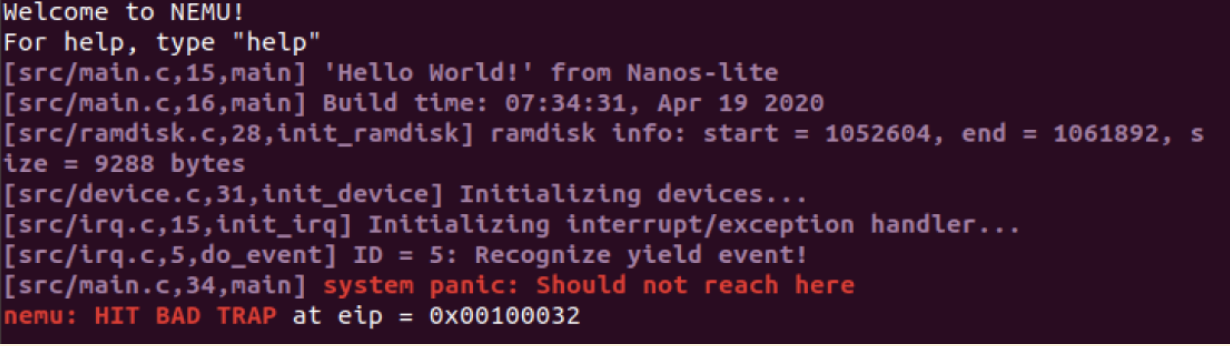
\includegraphics[scale=0.5]{fig/1.png}
        \caption{PA3.1结果}
    \end{figure}
}  
%---------------------------------------------------------------------------------------------------
\section{阶段二}
%——————————————————————————————————————
\subsection{加载用户程序}
\kt{
  显然批处理系统并不可能完全按照磁盘顺序依次执行,所以我们借助上述自陷操作要实现加载程序的功能模块。这一阶段的loader不需要对文件操作,所以简单的使用ramdisk提供的读盘API加载即可。之后再使用naive\_uload(NULL, NULL)加载makefile中定义的dummy即可。
  \begin{lstlisting}[title=loader1.0,frame=trbl,language={C++}]
uintptr_t loader(_Protect *as, const char *filename) {
  size_t size = get_ramdisk_size();
  void * buff = NULL;
  ramdisk_read(buff,0,size); 
  return (uintptr_t)DEFAULT_ENTRY;
}
  \end{lstlisting}
%——————————————————————————————————————
\subsection{YIELD和EXIT系统调用}
\kt{
    这里系统调用的实现实际上和前面的自陷操作流程是一致的,不过系统调用只需要ring3的用户级权限就可以了。这里指导书并没有像自陷操作一样非常详细,但实际上本质上是一样的,甚至还要更简单一些。过程大致为,中断发生,进入syscall入口程序,保护现场,根据系统调用号进行不同的处理,恢复现场,回到原来的调用处。所以实际上和yield是一样的。而当前步骤不需要对不同系统调用号进行不同处理。
    \begin{lstlisting}[title=syscall,frame=trbl,language={C++}]
//nexus-am/am/src/x86/nemu/cte.c
case 0x80:ev.event=_EVENT_SYSCALL;break;
//nanos-lite/src/irq.c
case _EVENT_SYSCALL:do_syscall(c);break;
//vecsys以及IDT的设置都已经有了就不需要管了
    \end{lstlisting}

    这个时候还是不对的,因为我们并没能很好的使用do\_syscall(),首先对arch.h里面的GPRx宏进行设定,让它们从上下文c中获得正确的系统调用参数寄存器,就可以用他们来实现syscall了,其实GPR1-4对应的是eax,ebx,ecx,edx,他们也正好分别代表系统调用号和参数。之后再在syscall.c中添加YIELD系统调用并设置正确返回值即可
    \begin{lstlisting}[title=yield,frame=trbl,language={C++}]
//nexus-am/am/include/arch/x86-nemu.h
#define GPR1 eax
#define GPR2 ebx
#define GPR3 ecx
#define GPR4 edx
#define GPRx eax
//nanos-lite/src/syscall.c
_Context* do_syscall(_Context *c) {
  uintptr_t a[4];
  a[0] = c->GPR1;
  a[1] =c->GPR2;
  a[2]=c->GPR3;
  a[3]=c->GPR4;
  switch (a[0]) {
    case SYS_yield:_yield();c->GPRx=0;break;
    case SYS_exit:_halt(a[1]);break;
  }
  return c;
}
    \end{lstlisting}
    以上都实现完成之后就可以看到程序运行Good\ Trap了。
    \begin{figure}[H]
      \centering
      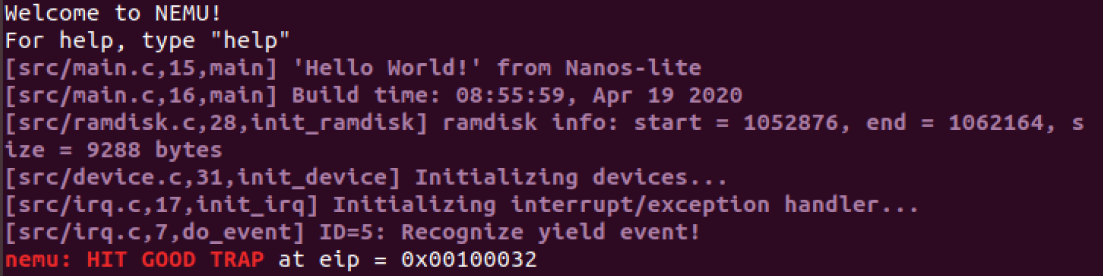
\includegraphics[scale=0.25]{fig/2.png}
      \caption{good trap}
  \end{figure}
}
%——————————————————————————————————————
\subsection{标准输出和堆区管理}
\kt{
    标准输出是OS必不可少的功能,像printf等都是通过调用sys\_write系统调用来实现标准输出的,而为了避免一个字符一个字符输出我们需要堆的帮助,这就需要sbrk的堆管理了。目前的sys\_write不涉及到文件写,只要根据文件描述符fd区分是否为stdout或strerr并调用\_putc输出即可,同时补全调用函数。
    \begin{lstlisting}[title=syswrite,frame=trbl,language={C++}]
//nanos-lite/src/syscall.c
static inline int32_t sys_write(int fd,const void *buf,size_t len)
{//实现简易版syswrite
  if(fd==1||fd==2){
    char *b=(char*)buf;
    printf("len is %d\n",len);
    for(int i=0;i<len;i++){
      _putc(*(b++));
    }
    return len;
  }
  return -1;
}
//系统调用号判别
case SYS_write:c->GPRx=sys_write(a[1],(void*)a[2],a[3]);break;
//navy-apps/libs/libos/src/nanos.c
int _write(int fd, void *buf, size_t count) {
  //_exit(SYS_write);
  return  _syscall_(SYS_write,fd,buf,count);
}
    \end{lstlisting}  

    之后就可以看到hello测试在进行printf的阶段每输出一个字符都会调用一次sys\_write,所以为了让程序有足够的内存空间使用,接下来实现堆的处理。
    \begin{figure}[H]
      \centering
      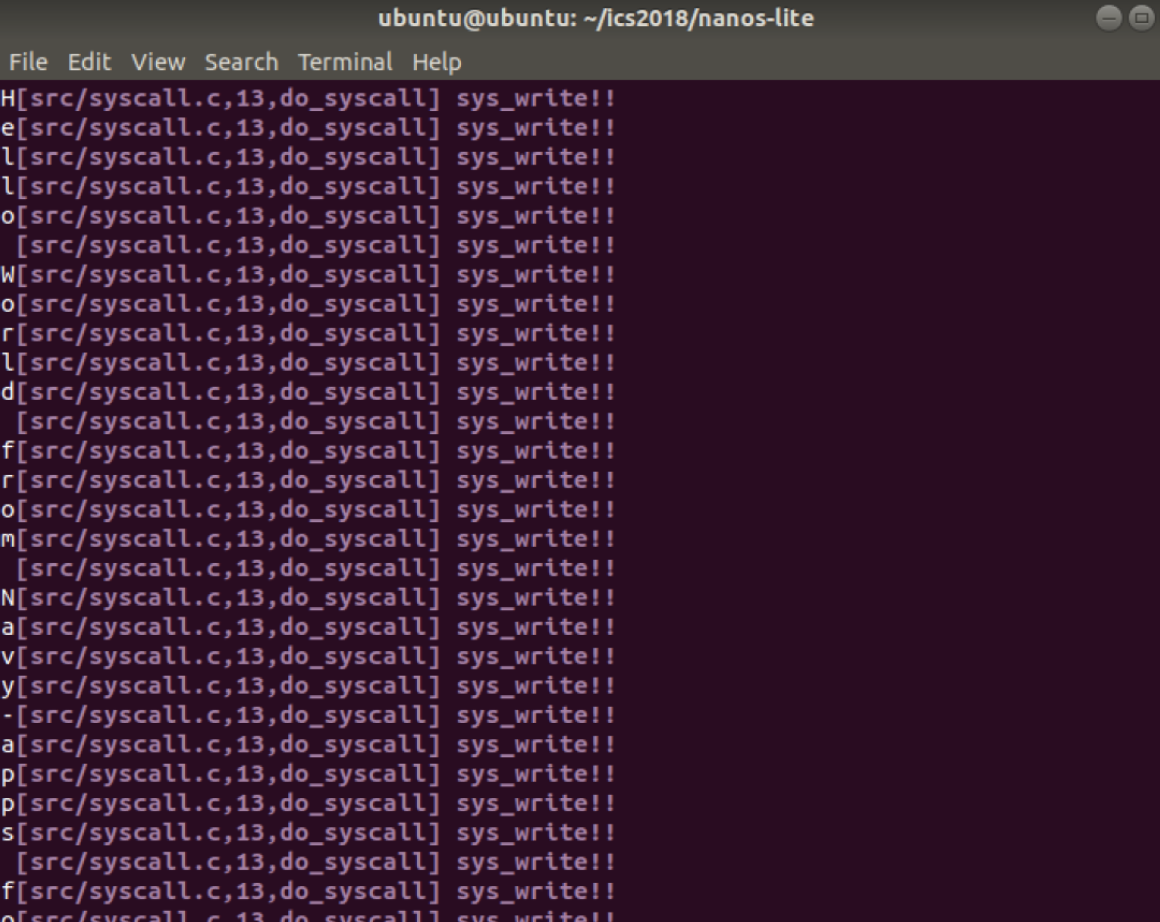
\includegraphics[scale=0.5]{fig/3.png}
      \caption{sys\_write}
  \end{figure}

  sys\_brk是用以设置堆区大小的系统调用,由于当前内存不受限制我们可以随意使用,所以该系统调用只要次次返回0,然后根据工作方式实现\_sbrk即可。这样printf就是一行一行的输出了。
  \begin{lstlisting}[title=sysbrk,frame=trbl,language={C++}]
//nanos-lite/src/syscall.c
  case SYS_brk:c->GPRx=0;break;
//navy-apps/libs/libos/src/nanos.c
void *_sbrk(intptr_t increment) {
    extern uint32_t _end;//pb初始位置
    static uint32_t program_break=&_end;
    if(_syscall_(SYS_brk,program_break+increment,0,0)==0)
    {//计算并设置新的pb
      uint32_t old=program_break;
      program_break=program_break+increment;
      return (void*)old;
    }
    else{//syscall失败
      return (void*)-1;
    }
  }
  \end{lstlisting}  
\begin{figure}[H]
    \centering
    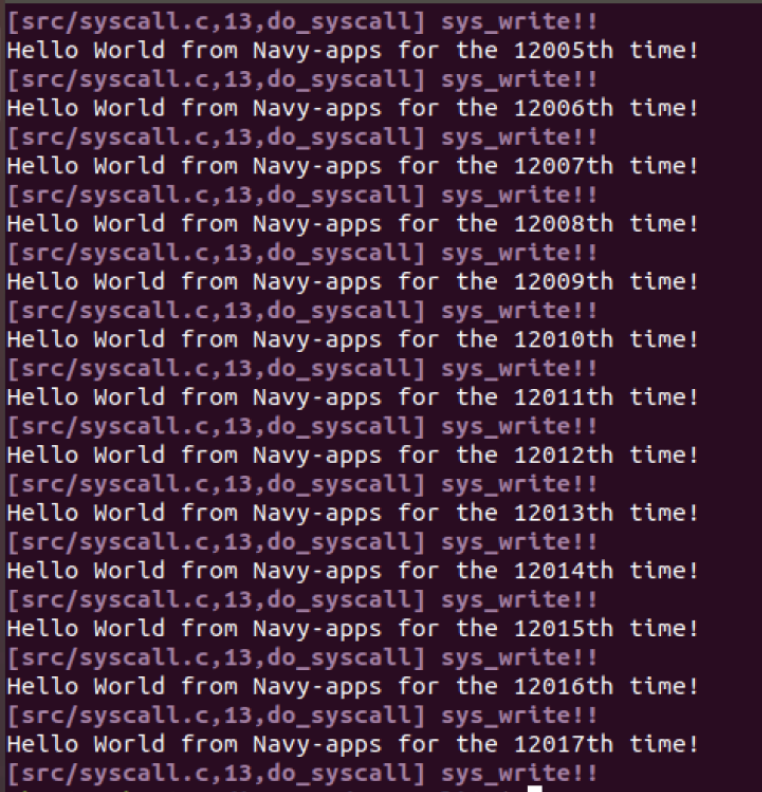
\includegraphics[scale=0.5]{fig/4.png}
    \caption{sys\_brk}
\end{figure}
}
%---------------------------------------------------------------------------------------------------
\section{阶段三}
%——————————————————————————————————————
\subsection{文件操作}
\kt{
  由于需要批处理系统执行的程序越来越多,单纯依靠磁盘就不够了,所以引入了文件系统,由于在PA中不需要多复杂,只要能支持批处理系统的基本功能就可以,且文件的大小和数量都是固定的,所以一些基本的读写操作等等就足矣。下面按照man给出信息一次实现文件操作函数。
  \begin{lstlisting}[title=文件操作,frame=trbl,language={C++}]
//nanos-lite/src/fs.c
off_t open_offset;//目前文件操作的位置,读写指针
size_t fs_filesz(int fd) {//获取文件大小
	return file_table[fd].size;
}
int fs_open(const char *pathname, int flags, int mode) 
{//读写任意文件,忽视flags和mode
	Log("Pathname: %s", pathname);
	int i;
	for (i = 0; i < NR_FILES; i++) {
		//printf("file name: %s\n", file_table[i].name);
		if (strcmp(file_table[i].name, pathname) == 0) {
			return i;
		}
	}
	return -1;
}
ssize_t fs_read(int fd, void *buf, size_t len) {
  ssize_t fs_size = fs_filesz(fd);
  //偏移量不可以超过文件边界 超出部分舍弃
	if (file_table[fd].open_offset + len > fs_size) 
		len = fs_size - file_table[fd].open_offset;
	switch(fd) {
		case FD_STDOUT:
		case FD_STDERR:
		case FD_STDIN:
			return 0;
		default:
      ramdisk_read(buf, file_table[fd].disk_offset + 
      file_table[fd].open_offset, len);
			file_table[fd].open_offset += len;
			break;
	}
	return len;
}
ssize_t fs_write(int fd, const void *buf, size_t len) {
	ssize_t fs_size = fs_filesz(fd);
	switch(fd) {
		case FD_STDOUT:
		case FD_STDERR:
			for(int i = 0; i < len; i++) {
				_putc(((char*)buf)[i]);
			}
			break;
		default:
			if(file_table[fd].open_offset + len > fs_size)
				len = fs_size - file_table[fd].open_offset;
			// 对文件的真正读写
      ramdisk_write(buf, file_table[fd].disk_offset +
       file_table[fd].open_offset, len);
			file_table[fd].open_offset += len;
			break;
	}
	return len;// 参见man 返回值
}
off_t fs_lseek(int fd, off_t offset, int whence) {
	off_t result = -1;
	// man 2 lseek 注意边界!
	switch(whence) {
		case SEEK_SET://open设置为offset
			if (offset >= 0 && offset <= file_table[fd].size) {
				file_table[fd].open_offset = offset;
				result = file_table[fd].open_offset;
			}
			break;
		case SEEK_CUR://open=current+offset
      if ((offset + file_table[fd].open_offset >= 0) 
      && (offset + file_table[fd].open_offset 
      <= file_table[fd].size)) {
				file_table[fd].open_offset += offset;
				result = file_table[fd].open_offset;
			}
			break;
		case SEEK_END://open=文件大小+offset
			file_table[fd].open_offset = file_table[fd].size + offset;
			result = file_table[fd].open_offset;
			break;
	}
	return result;
}
int fs_close(int fd) {
	return 0;
}
    \end{lstlisting}

    除了fs.c中的内容,我们还需要实现各种文件相关的系统调用才能使文件系统正常工作:
    \begin{lstlisting}[title=文件系统调用,frame=trbl,language={C++}]
//nanos-lite/src/syscall.c 
case SYS_open:c->GPRx=fs_open((void*)a[1],a[2],a[3]);break;
case SYS_read:c->GPRx=fs_read(a[1],(void*)a[2],a[3]);break;
case SYS_write:c->GPRx=fs_write(a[1],(void*)a[2],a[3]);break;
case SYS_close:c->GPRx=fs_close(a[1]);break;
case SYS_lseek:c->GPRx=fs_lseek(a[1],a[2],a[3]);break;
//navy-apps/libs/libos/src/nanos.c
int _open(const char *path, int flags, mode_t mode) {
  //_exit(SYS_open);
  return _syscall_(SYS_open,path,flags,mode);
}int _read(int fd, void *buf, size_t count) {
  //_exit(SYS_read);
  //printf("%d\n",count);
  return _syscall_(SYS_read,fd,buf,count);
}

int _close(int fd) {
  //_exit(SYS_close);
  return _syscall_(SYS_close,fd,0,0);
}

off_t _lseek(int fd, off_t offset, int whence) {
  //_exit(SYS_lseek);
  return _syscall_(SYS_lseek,fd,offset,whence);
}
    \end{lstlisting}
    
    之后再用naive\_uload加载text测试,可以看到如下结果:
    \begin{figure}[H]
        \centering
        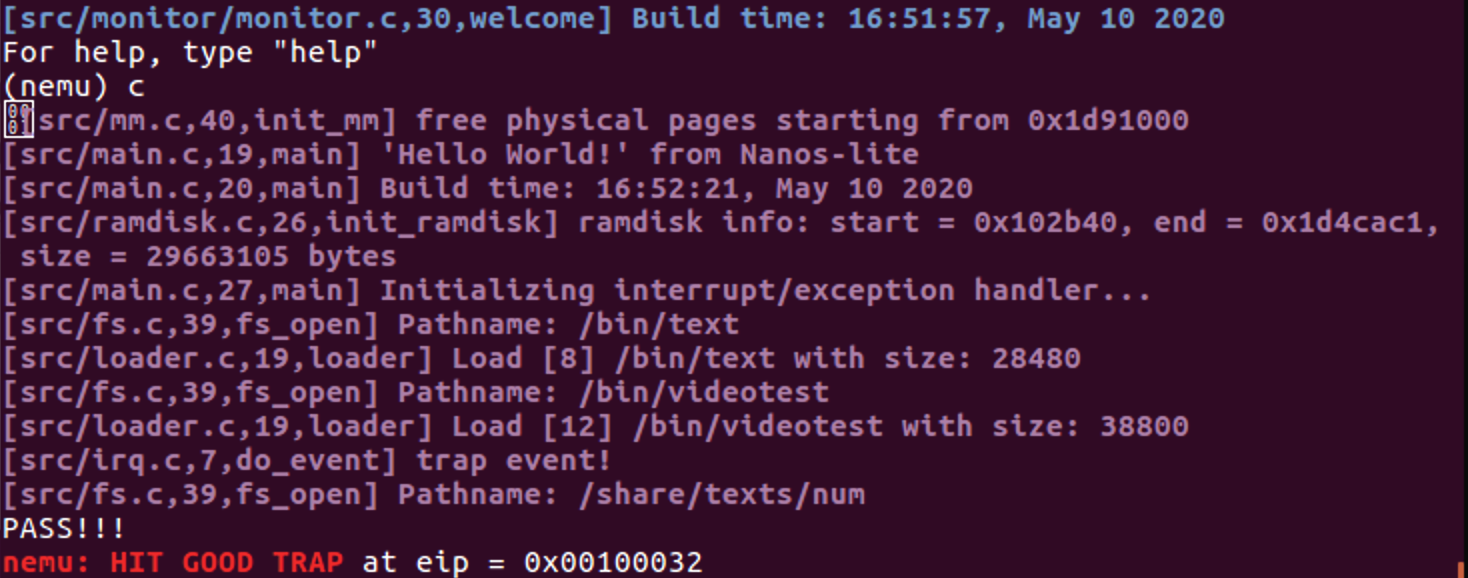
\includegraphics[scale=0.45]{fig/5.png}
        \caption{PASS!!}
    \end{figure}
}
%——————————————————————————————————————
\subsection{万物皆文件}
\kt{
    接下来的部分是继续完善文件系统的功能,如前面PA2.3实现的一些IO功能,键盘输入,VGA 等等。

    串口的写入在device.c中由serial\_write()提供,实现该函数并完善VFS即可,原理还是putc。

    读取输入事件的实现,步骤和串口写入一致,完成events\_read()函数并完善VFS。
    \begin{lstlisting}[title=serial\&events,frame=trbl,language={C++}]
//nanos-lite/src/device.c 
size_t serial_write(const void *buf, size_t offset, size_t len) 
{//串口写入
  char *b=(char*)buf;
  for(int i=0;i<len;i++){
    _putc(*(b++));
  }
  return len;
}
size_t events_read(void *buf, size_t offset, size_t len) 
{//输入事件
  int key=read_key();
    if(key & 0x8000){
        sprintf(buf,"kd %s\n",keyname[key & ~0x8000]);
    }
    else if ((key & ~0x8000)!=_KEY_NONE){
        sprintf(buf,"ku %s\n",keyname[key & ~0x8000]);
    }
    else{
      sprintf(buf,"t %d\n",uptime());
    }
  return strlen(buf);
}
//nanos-lite/src/fs.c 
static Finfo file_table[] __attribute__((used)) = {
  {"stdin", 0, 0, 0,invalid_read, invalid_write},
  {"stdout", 0, 0, 0,invalid_read, serial_write},
  {"stderr", 0, 0, 0,invalid_read, serial_write},
#include "files.h"
  {"/dev/events",0,0,0,events_read,invalid_write},
  {"/dev/fbsync",1,0,0,invalid_read,fbsync_write},
  {"/dev/tty",0,0,0,invalid_read,serial_write},
  {"/proc/dispinfo",0,0,0,dispinfo_read,invalid_write},
  {"/dev/fb",0,0,0,invalid_read,fb_write},
};
  \end{lstlisting}

  VGA抽象成文件,需要对frame\ buffer的大小进行初始化,并实现写屏幕的相关函数,同时完善VFS。
  \begin{lstlisting}[title=serial\&events,frame=trbl,language={C++}]
//nanos-lite/src/fs.c 
void init_fs() {
  // TODO: initialize the size of /dev/fb
  file_table[FD_FB].size = _screen.height * _screen.width * 4;
}
//nanos-lite/src/device.c 
size_t fb_write(const void *buf, size_t offset, size_t len) 
{//根据offset计算xy再调用draw_rect
  int x=(offset/4)%screen_width(); 
  int y=(offset/4)/screen_width();
  draw_rect((uint32_t*)buf,x,y,len/4,1);
  return len;
}
size_t fbsync_write(const void *buf, size_t offset, size_t len) 
{//调API
  draw_sync();
  return 0;
}
//初始化/proc/dispinfo
void init_device() {
  Log("Initializing devices...");
  _ioe_init();

  // TODO: print the string to array `dispinfo` with the format
  // described in the Navy-apps convention
  sprintf(dispinfo,"WIDTH:%d\nHEIGHT:%d\n",screen_width(),screen_height());
}
size_t dispinfo_read(void *buf, size_t offset, size_t len) {
  strncpy(buf,dispinfo+offset,len);
  return len;
}
  \end{lstlisting}

  以上内容都成功实现后,对events和bmptest测试就可以看到预期的结果。
\begin{figure}[H]
    \centering
    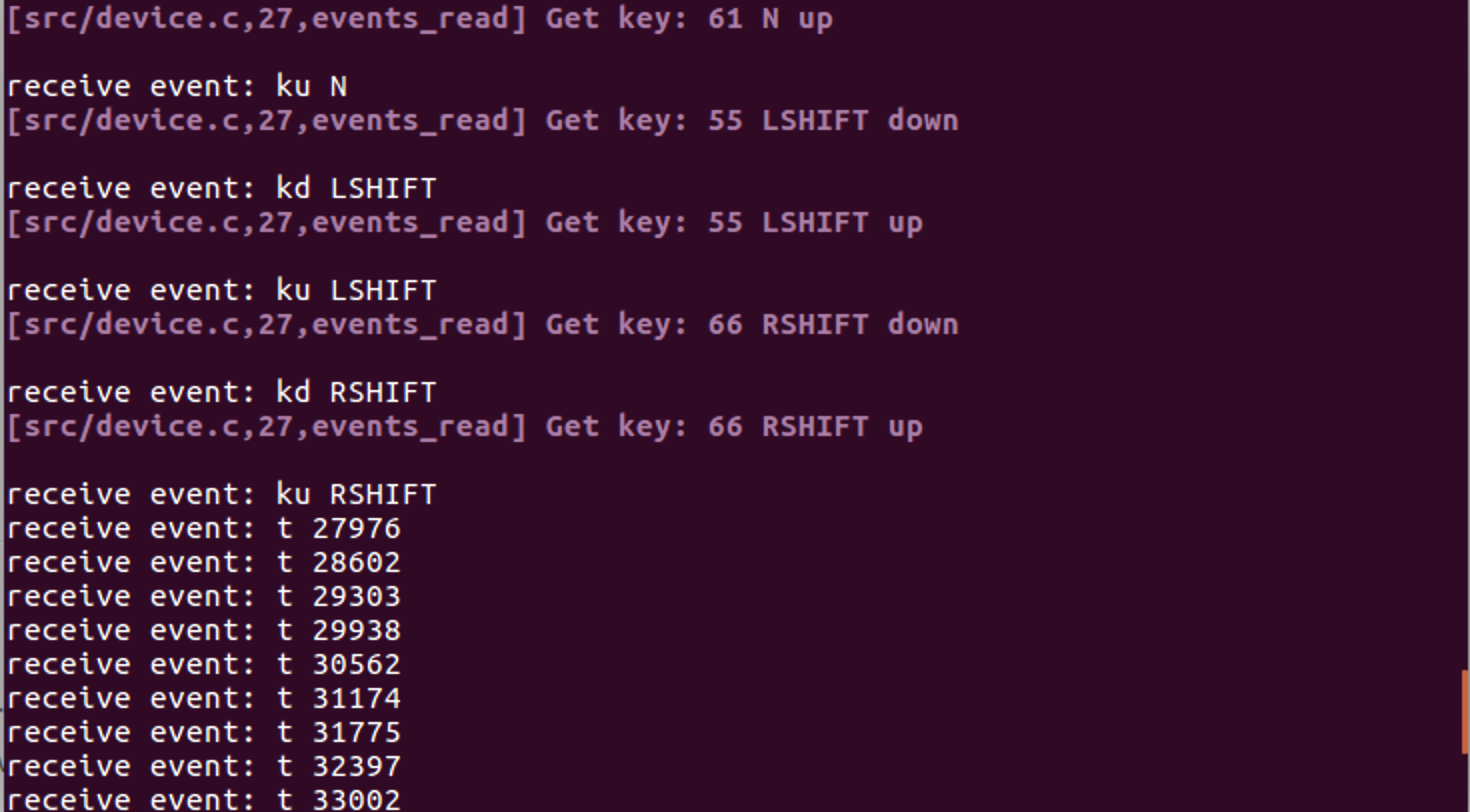
\includegraphics[scale=0.45]{fig/6.png}
    \caption{events}
\end{figure}
\begin{figure}[H]
  \centering
  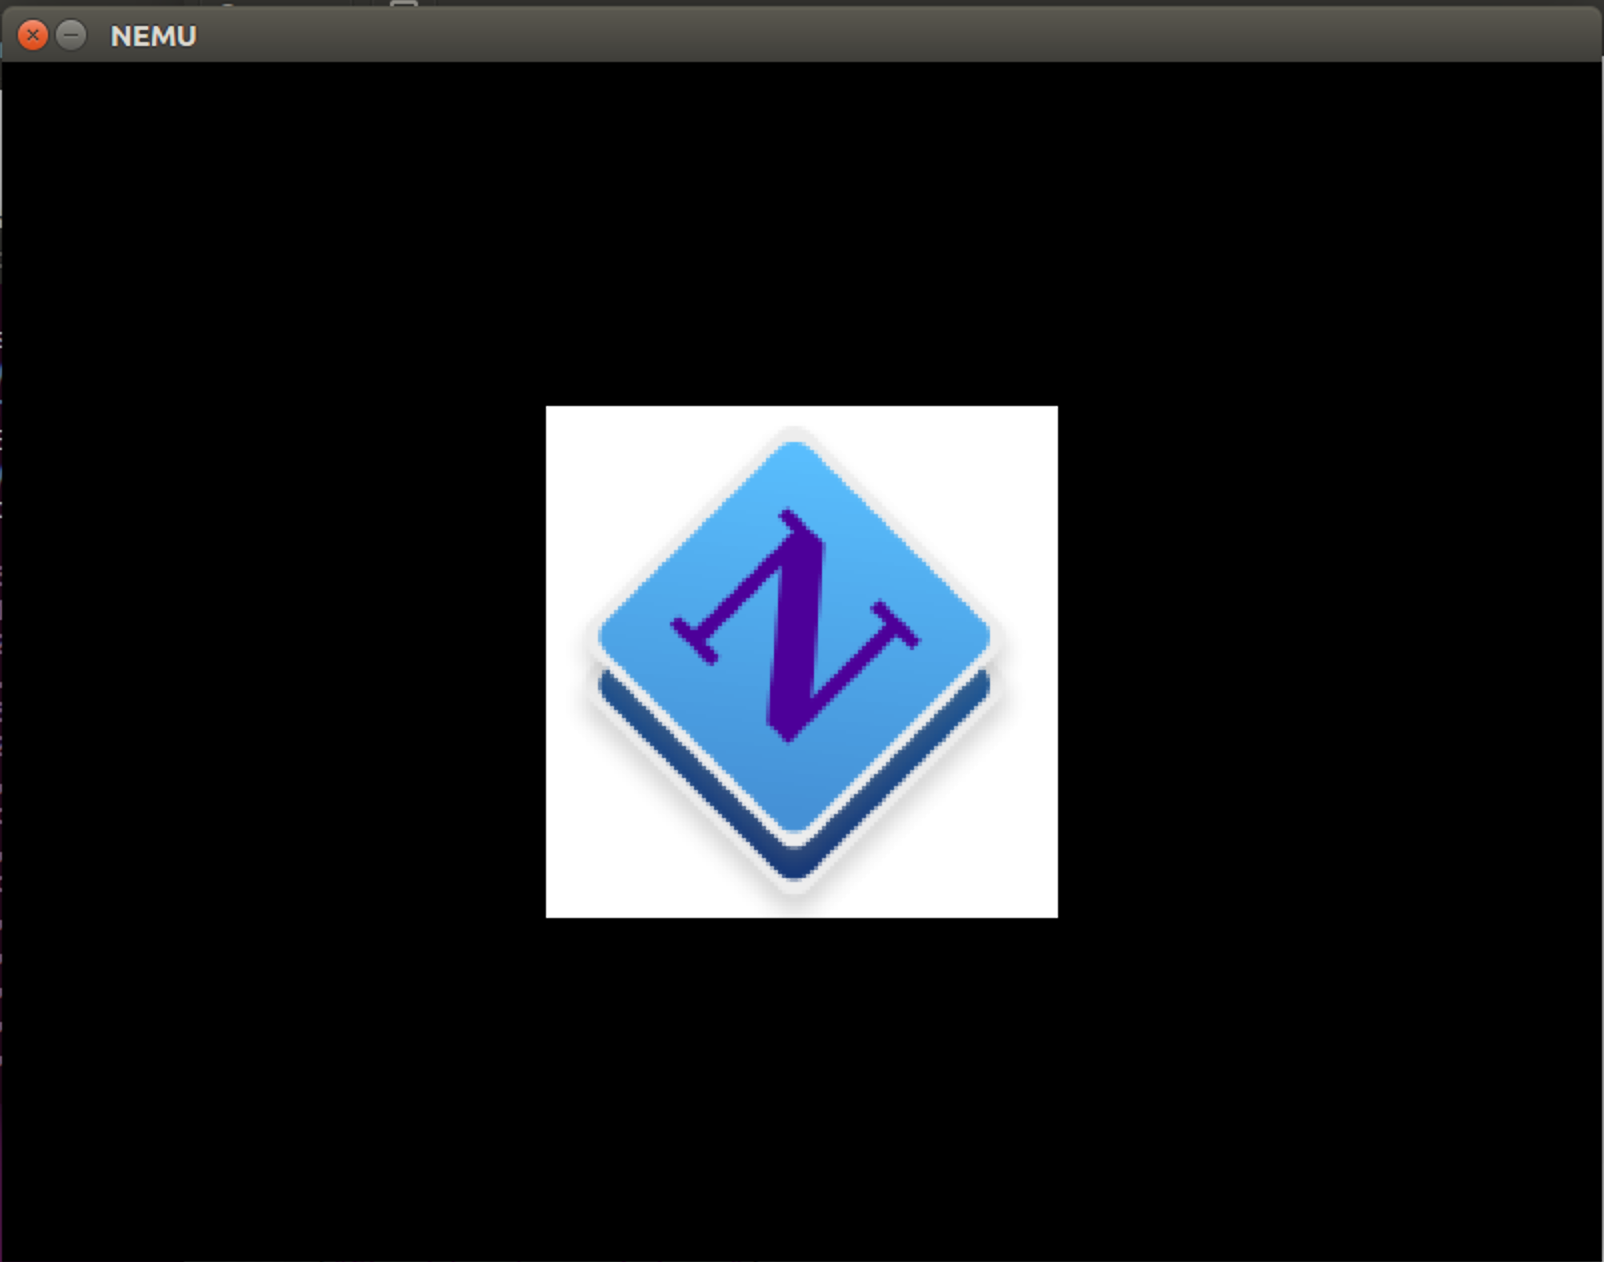
\includegraphics[scale=0.45]{fig/7.png}
  \caption{bmptest}
\end{figure}
}
%——————————————————————————————————————
\subsection{运行仙剑}
\kt{
  仙剑前面都实现完了之后,仙剑就可以直接运行了。但是NEMU真的慢到承受不住,假装前面都没什么问题吧就。。。由于浮点数还没有实现所以还不可以战斗,但其实到水月宫战斗前的剧情还是挺长的,只不过太慢了完全等不到那么久,运行到去菜市场就假装这里已经好了orz,此时的存档似乎也不是很好用,可能是mmu还没有实现的原因。
    \begin{figure}[H]
        \centering
        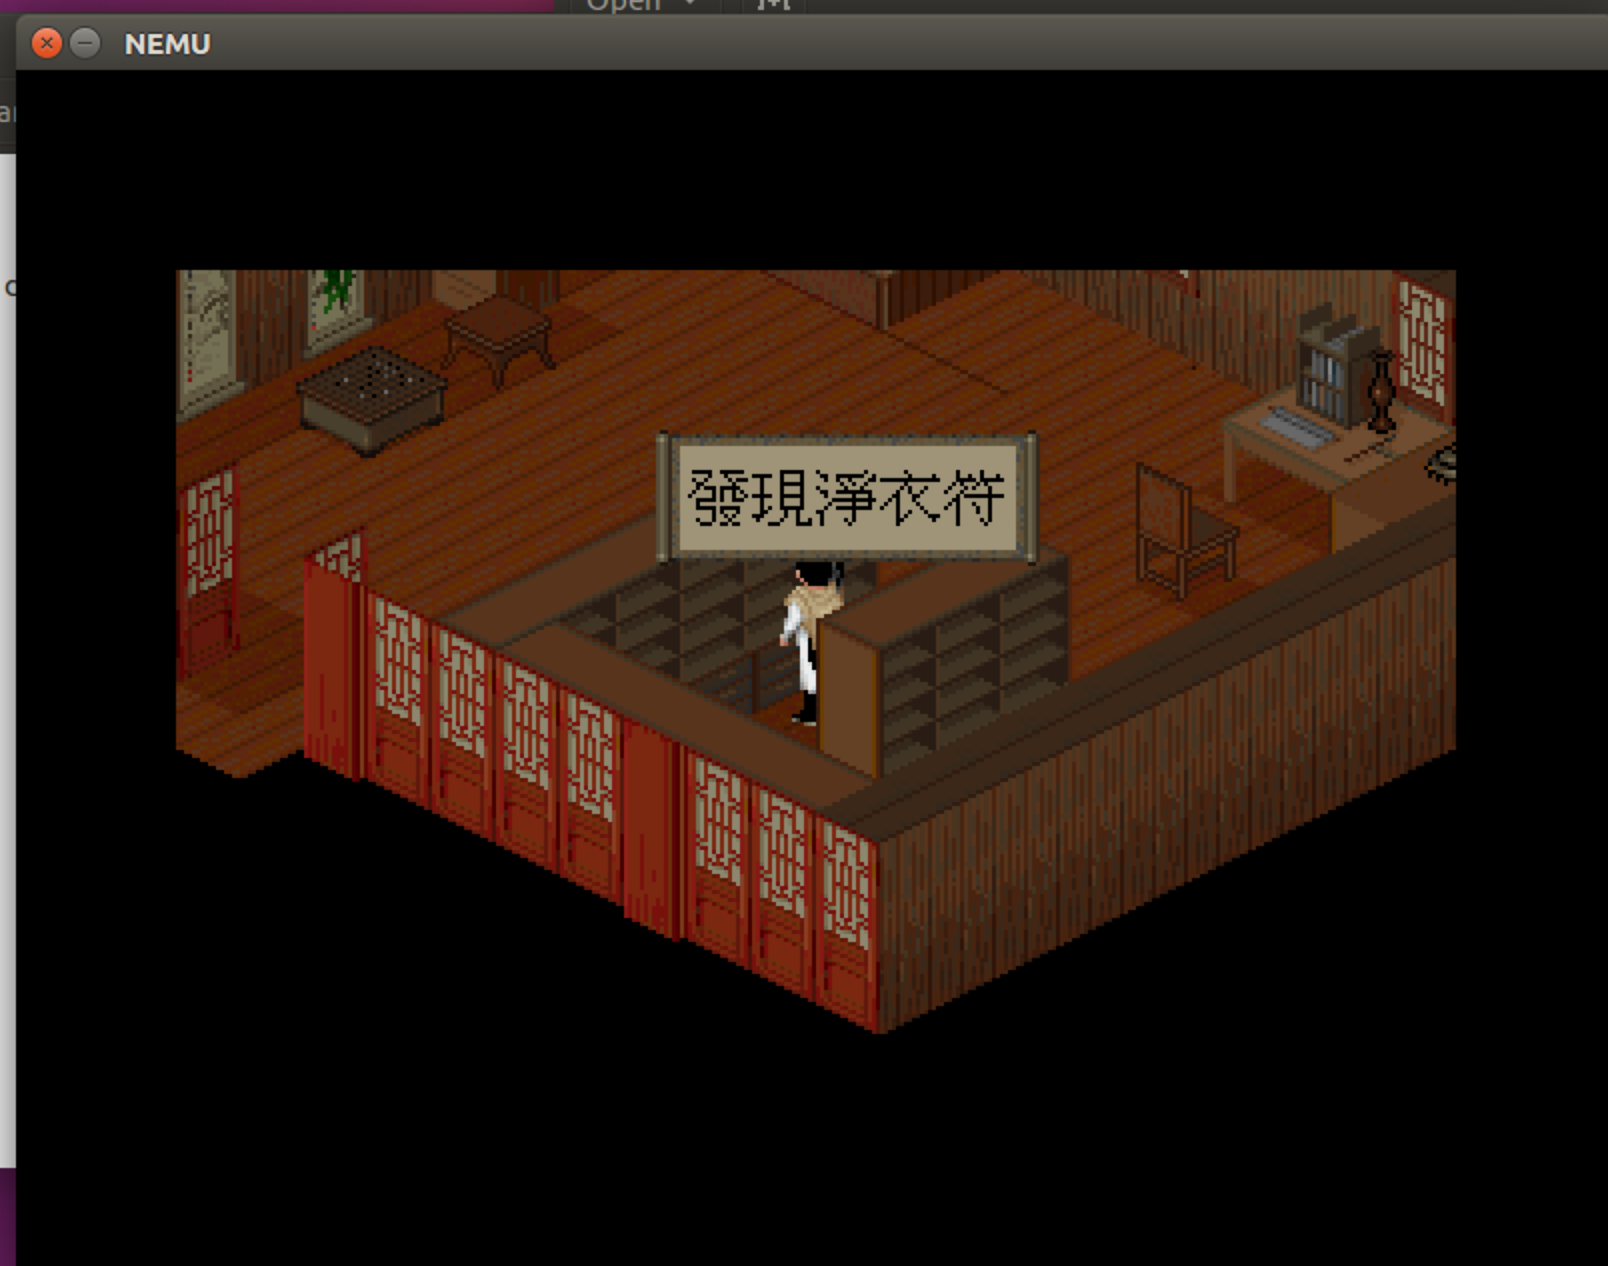
\includegraphics[scale=0.45]{fig/8.png}
        \caption{pal}
    \end{figure}
}
%——————————————————————————————————————
\subsection{DiffTest}
\kt{
    实际上2019的框架已经非常齐全了,只需要去掉运行参数-b,这里2019实验书写的路径是错误的,应该是在nexus-am\/am\/arch\/platform\/nemu.mk里面,然后在monitor里面实现detach和attach两个命令,并对EFLAGS和IDTR这两个寄存器进行处理,以跳过这些和QEMU真机不太一样的地方。
    \begin{lstlisting}[title=difftest,frame=trbl,language={C++}]
//nemu/src/monitor/ui.c
/*cmd_table加入描述*/
{ "detach", "Exit DiffTest", cmd_detach},//New
{ "attach", "Attach DiffTest with Qemu", cmd_attach},//New
/*命令实现*/
static int cmd_detach(char *args){
  difftest_detach();
  return 0;
}
static int cmd_attach(char *args){
  difftest_attach();
  return 0;
}
//nemu/src/monitor/diff-test.c
void difftest_detach() {
  is_detach = true;
}
void difftest_attach() {
#ifndef DIFF_TEST
  return;
#endif
  is_detach = false;
  is_skip_ref = false;
  skip_dut_nr_instr = 0;
  isa_difftest_attach();
}
//nemu/tools/qemu-diff/src/isa/x86/init.c
r.eip = 0x7c00;
r.cs = 0x0000;
ok = gdb_setregs(&r);
assert(ok == 1);
    \end{lstlisting}
   
}
%——————————————————————————————————————
\subsection{展示批处理系统}
\kt{
  实现execve系统调用使得结束当前程序运行的时候启动一个指定的程序,借助它来实现开始菜单,并修改exit系统调用使得程序运行结束的时候回到开始菜单。之后运行超级玛丽比仙剑能快那么一点点吧。。
  \begin{lstlisting}[title=execve,frame=trbl,language={C++}]
//nanos-lite/src/syscall.c
case SYS_exit:c->GPRx=-1;naive_uload(NULL,"/bin/init");break;//_halt(a[1]);break;
case SYS_execve:c->GPRx=-1;naive_uload(NULL,(char*)a[1]);break;
  \end{lstlisting}
  \begin{figure}[H]
    \centering
    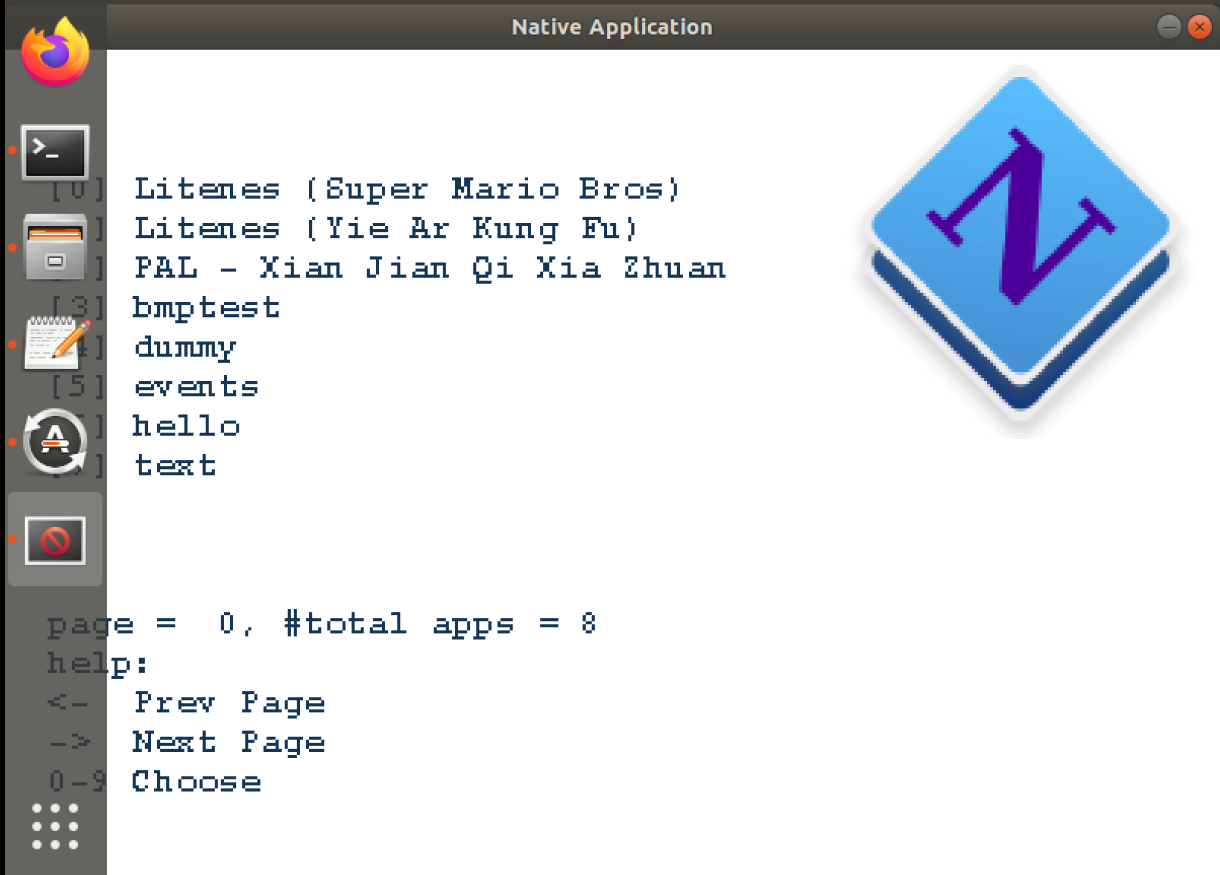
\includegraphics[scale=0.25]{fig/9.png}
    \caption{批处理主界面}
\end{figure}

由于马里奥运行出来的结果和以前没什么两样就不放图了。
}
%---------------------------------------------------------------------------------------------------
\section{遇到的bug及解决}
\kt{
    PA3重写了三次,最后在PA4的时候还是因为太菜回到了2018,放弃了在2019的苦苦挣扎,幸好PA4没有再重写。
    \begin{itemize}
        \item 
        \begin{todolist}
            \item [\done] 不知道是我理解的问题还是实验书表达的有一点点问题,3.2的时候应该是要现在loader里面实现加载磁盘文件才可以继续后面系统调用等等的完善,不然一定会卡住;同样的理解问题,实验指导书说“trap.S中实现的结构”但是trap.S根本就没写,所以意思应该是trap.S中使用的构造的上下文结构的顺序
            \item [\done] 2019新增的那个logo从一开始的运行就开始报地址的错,然后等我把logo.txt的图标大小改小一点就好了?后面好像是因为文件读写长度的问题?等我文件系统改好以后这个就没有问题了
            \item [\done] lidt指令里面用的是id\_dest的地址不是val
            \item [\done] text测试样例那里应该是要先写好serial\_write才可以
            \item [\done] PA3发现了不少PA2留下的小坑以及没有补充完整的opcode\_table,还有PA3的内容我都是先行在native测试的,确定nanos-lite的实现没有问题再找前面遗留下的问题
            \item 其实仙剑还是有点问题的,不止是战斗无法进行,我的剧情在地图切换后就出现了问题(买鱼没买到回来)就环境变暗卡住了,但是直到PA5才发现是前面的指令实现有问题orz,除了感谢我对仙剑剧情倒背如流能告诉小伙伴正确的剧情操作顺序以外,并让我一下子就知道哪里有bug,但是这蜗牛爬的运行速度我实在不想改(实际上PA3测试的部分到要出客栈门就再没管,因为太慢了这就半个小时了,直觉感官上甚至比零几年的xp机还慢)
        \end{todolist}
    \end{itemize}
}
%---------------------------------------------------------------------------------------------------
\section{思考题\&\&必答题}
%——————————————————————————————————————
\subsection{思考题}
\kt{
    \begin{enumerate}
        \item 什么是操作系统
        
        这个问题我只能抄网上,属于只可意会表达不出的概念。操作系统位于计算机硬件与应用软件之间,本质也是一个软件。操作系统由操作系统的内核(运行于内核态,管理硬件资源)以及系统调用(运行于用户态,为应用程序员写的应用程序提供系统调用接口)两部分组成。

        操作系统的功能是:进程管理,其主要任务是对处理器的时间进行合理分配、对处理器的运行实施有效的管理;存储器管理,主要任务是对存储器进行分配、保护和扩充;设备管理,根据确定的设备分配原则对设备进行分配,使设备与主机能够并行工作,为用户提供良好的设备使用界面;文件管理,有效地管理文件的存储空间,合理地组织和管理文件系统,为文件访问和文件保护提供更有效的方法及手段;用户接口,通过用户接口,用户只需进行简单操作,就能实现复杂的应用处理。
        
        如果放在NEMU上来看,操作系统就是运行在AM上的一个特殊的程序,他可以加载其他程序对他们进行资源分配和管理等等。
        \item 这些程序状态(x86的eflags, cs, eip; mips32的epc, status, cause; riscv32的sepc, sstatus, scause)必须由硬件来保存吗? 能否通过软件来保存? 为什么?
        
        软件崩了不就找不回来了
        \item 我们知道进行函数调用的时候也需要保存调用者的状态: 返回地址, 以及calling convention中需要调用者保存的寄存器. 而CTE在保存上下文的时候却要保存更多的信息. 尝试对比它们, 并思考两者保存信息不同是什么原因造成的.
        
        在函数调用过程中,寄存器被分为调用者保存寄存器和被调用者保存寄存器,由于框架作出了相应的规定,调用者保存寄存器依情况保存,而在异常处理时,处于内核态,操作系统拥有最高的权限,可以使用更改任何寄存器,而标志寄存器这些与程序的运行状态息息相关,所以要保存所以寄存器。
        \item x86的trap.S中有一行pushl \%esp的代码, 乍看之下其行为十分诡异. 你能结合前后的代码理解它的行为吗? Hint: 不用想太多, 其实都是你学过的知识.
        
        call指令压栈esp,查看irq\_handle(\_RegSet *tf),可能是在准备入口参数call指令执行完后,执行了esp+4,使esp指向了进入陷阱帧之前的位置,还原了陷阱帧调用前的函数状态
        \item 如果你在GNU/Linux下执行一个从Windows拷过来的可执行文件, 将会报告"格式错误". 思考一下, GNU/Linux是如何知道"格式错误"的?
        
        文件头中包含的文件描述符等信息的无法识别等导致的格式错误出现
        \item 使用readelf查看一个ELF文件的信息, 你会看到一个segment包含两个大小的属性, 分别是FileSiz和MemSiz, 这是为什么? 再仔细观察一下, 你会发现FileSiz通常不会大于相应的MemSiz, 这又是为什么?
        
        分别表示文件大小和在内存中占据空间大小,那必然文件大小会小
        \item 在navy-apps/apps/pal/src/game/script.c中有一个PAL\_InterpretInstruction()的函数, 尝试大致了解这个函数的作用和行为. 然后大胆猜测一下, 仙剑奇侠传的开发者是如何开发这款游戏的? 你对"游戏引擎"是否有新的认识?
        
        大胆胡乱猜测如下,该函数用以解释和执行脚本文件中的各个指令。对于不同的操作码对应不同的游戏行为,大概就是借助这个神奇的形似CPU exec部分的对游戏内不同操作码进行翻译和执行。这就大概是个游戏引擎吧。。
        \item 假设这些上述这些秘技并非游戏制作人员的本意, 请尝试解释这些秘技为什么能生效.
        
        其实这三个秘技我只尝试成功过后两个,第一个不知道什么原因玩了几次都没有成功,再就是网上有不少修改器可以穿墙感觉是同一个原理,可能是和程序实现中没有考虑临界值的计算以及类型转换导致的数据溢出,导致如二号人物赵灵儿的技能也处于一号人物李逍遥的技能范围内了。
    \end{enumerate}
}
%——————————————————————————————————————
\subsection{必答题}
\kt{
    以下以外的必答题均为代码实现。
    \begin{enumerate}
        \item 你会在\_\_am\_irq\_handle()中看到有一个上下文结构指针c, c指向的上下文结构究竟在哪里? 这个上下文结构又是怎么来的? 具体地, 这个上下文结构有很多成员, 每一个成员究竟在哪里赋值的? \$ISA-nemu.h, trap.S, 上述讲义文字, 以及你刚刚在NEMU中实现的新指令, 这四部分内容又有什么联系?
        
        指向的结构体在esp指向的地方,这个结构体是是前面pushal构造的,其成员的定义在x86-nemu.h中,包括地址空间、通用寄存器、irq、eip、cs以及eflags,irq的赋值在trap.S中对应不同中断事件pushal对寄存器操作,然后是eip、eflags。x86-nemu.h定义了context,trap.S是中断发生时的处理过程,实现的popa指令用来恢复trapframe
        \item 从Nanos-lite调用\_yield()开始, 到从\_yield()返回的期间, 这一趟旅程具体经历了什么? 软(AM, Nanos-lite)硬(NEMU)件是如何相互协助来完成这趟旅程的? 你需要解释这一过程中的每一处细节, 包括涉及的每一行汇编代码/C代码的行为, 尤其是一些比较关键的指令/变量. 事实上, 上文的必答题"理解上下文结构体的前世今生"已经涵盖了这趟旅程中的一部分, 你可以把它的回答包含进来.别被"每一行代码"吓到了, 这个过程也就大约50行代码, 要完全理解透彻并不是不可能的. 我们之所以设置这道必答题, 是为了强迫你理解清楚这个过程中的每一处细节. 这一理解是如此重要, 以至于如果你缺少它, 接下来你面对bug几乎是束手无策.

        首先\_yield在cte.c中实现是通过int\ 81实现的,int指令借助raise\_intr实现对中断号81的处理,根据trap.S将上下文设置好之后调用\_\_am\_irq\_handle,按照前面对事件的标号进行处理(输出一句话)然后返回并恢复上下文,再返回到调用\_yield的地方。
        \item 我们知道navy-apps/tests/hello/hello.c只是一个C源文件, 它会被编译链接成一个ELF文件. 那么, hello程序一开始在哪里? 它是怎么出现内存中的? 为什么会出现在目前的内存位置? 它的第一条指令在哪里? 究竟是怎么执行到它的第一条指令的? hello程序在不断地打印字符串, 每一个字符又是经历了什么才会最终出现在终端上?
        
        程序编译出之后在hello文件夹下的build文件夹里,出现的具体步骤见Makefile.app是链接所有库文件之后编译生成的ELF文件,因为Makefile里设定了它要放在这里,ELF的header之后就是,根据加载的ELF文件,其头部中指示了代码段的位置即可执行,经历了不停的调用write和brk

    \end{enumerate}
}
%----------------------------------------------------------------------------- 
\section{总结}
\kt{
    
    PA3代码感觉不多但是却处处致命,虽然挺早就写完了PA3但是直到PA5我还发现了PA2和PA3的一些小问题,费时在自己给自己挖坑上。
    
    虽然整体时间不是很长,但是如果算上后面部分的调试时间还是有些多,只能怪罪于自己没能完全理解实验报告,或者基础理论知识还不够透彻上吧。Difftest虽然提前写好了但其实没怎么用,还是靠着报错提示去找,因为difftes的实现在PA3阶段还有点小问题(和QEMU的协同上)。

    整体上又跟随PA成长了许多,但是拿仙剑做例子总是让人忍不住去玩,幸好NEMU极慢极慢的运行打消了我这个念头,然后PA5的优化目前并没有什么头绪,希望在重览实验指导后能摸清一些门路。
}
%----------------------------------------------------------------------------- 
% \lhead{\kaishu 参考文献}
% \newpage
% \kt{
% \begin{thebibliography}{plain}  
%     \bibitem{ref1}Ray Tracing经典入门[EB/OL].https://raytracing.github.io/books/
%     \bibitem{ref2}讲稿lec2-5,8
% \end{thebibliography}
% }
\end{document}
